% \section{Appendix}
% \label{sec:append}



\section{Improving the precision of the large spheres}
\label{subsec:Improve_Large} Recall that for each large circle $C_{i}\in\C_{L}^{*}$
we guessed its center in the optimal packing up to a polynomial error
of $\frac{\eps}{n}$. We improve this to only an exponential error
of at most $\frac{1}{2^{n/\eps}}$. To do this, we apply Theorem~\ref{thm:GrigorevVV88}
with $\alpha:=\Theta(\frac{1}{2^{n/\eps}})$. This yields more precise
estimates $\bar{x}_{i}^{(1)},\bar{x}_{i}^{(2)}$ for each $C_{i}\in\C_{L}^{*}$.
There is an important subtlety though: for our guessed coordinates
$\tilde{x}_{i}^{(1)},\tilde{x}_{i}^{(2)}$ we can assume that they
differ from the coordinates of $\OPT$ by at most our polynomial error
of $\frac{\eps}{n}$. For the new estimates $\bar{x}_{i}^{(1)},\bar{x}_{i}^{(2)}$
we can \emph{not }guarantee this: our subroutine from Theorem~\ref{thm:GrigorevVV88}
possibly returns a solution that is (close to) a feasible for the
large circles, but not (close to) a solution that is feasible for
the large and for the small circles. Because of this, we guessed the estimates
$\tilde{x}_{i}^{(1)},\tilde{x}_{i}^{(2)}$ for each $C_{i}\in\C_{L}^{*}$,
so that we can assume that these estimates really correspond to $\OPT$
and not just to some arbitrary solution to \eqref{eq:equations}.

If it were true that there is always a $(1+\eps)$-approximate solution
in which the center of each circle has rational coordinates that can
be encoded with a polynomially bounded number of bits, then we could
choose $\alpha$ appropriately to compute it. More precisely, we could
compute a range for each coordinate that contains only one rational
number with a bounded number of bits, and we could compute this number
afterward.



%
%
% \label{subsec:Improve_Large}
% So far, for each large circle $C_{i}\in\C_{L}^{*}$ we guessed values
% $\tilde{x}_{i}^{(1)},\tilde{x}_{i}^{(2)}\in\{0,\frac{\eps}{n},\frac{2\eps}{n},...,1\}$
% such that $\hat{x}_{i}^{(1)}\in[\tilde{x}_{i}^{(1)},\tilde{x}_{i}^{(1)}+\frac{\eps}{n})$
% and $\hat{x}_{i}^{(2)}\in[\tilde{x}_{i}^{(2)},\tilde{x}_{i}^{(2)}+\frac{\eps}{n})$.
% Hence, we possibly make a polynomial error of $\frac{\eps}{n}$.
% We improve this to only an exponential error of at most
% $\frac{1}{2^{n/\eps}}$. To do this, we apply Theorem~\ref{thm:GrigorevVV88} with
% $\alpha:=\Theta(\frac{1}{2^{n/\eps}})$. This yields more precise estimates
% $\bar{x}_{i}^{(1)},\bar{x}_{i}^{(2)}$ for each $C_{i}\in\C_{L}^{*}$.
% However, note that it
% might \emph{not} be the case that
% $\hat{x}_{i}^{(1)}\in[\bar{x}_{i}^{(1)},\bar{x}_{i}^{(1)}+\frac{1}{2^{n/\eps}})$
% and
% $\hat{x}_{i}^{(2)}\in[\bar{x}_{i}^{(2)},\bar{x}_{i}^{(2)}+\frac{1}{2^{n/\eps}})$
% for some $C_{i}\in\C_{L}^{*}$. The reason is that
% our system of inequalites~\eqref{eq:equations} can have solutions that differ from
% $\hat{x}_{i}^{(1)},\hat{x}_{i}^{(2)}$ for some (or even all) large circles $C_{i}\in\C_{L}^{*}$. Because of
% this, we guessed the estimates $\tilde{x}_{i}^{(1)},\tilde{x}_{i}^{(2)}$ for each $C_{i}\in\C_{L}^{*}$, so that
% we can assume that these estimates correspond to $\OPT$ and not just to some arbitrary solution to \eqref{eq:equations}.
%
% If it were true that there is always a $(1+\eps)$-approximate solution
% in which the center of each circle has rational coordinates that can be encoded with a polynomially bounded number of bits,
% then we could choose $\alpha$ appropriately to compute it. More precisely, we could compute a range for each coordinate that contains only one
% rational number with a bounded number of bits, and we could compute this number afterward.


\section{Shifting step}\label{sec:shifting}
%\begin{restatable}{lem}{shiftinglemmaapx}
\begin{lem}
	\label{lem:shifting}
	Let a given packing for a knapsack packing problem with input set \(\C\) of items be $\mathcal{P}$ and \(r\) be a total order on these objects and \(w_i\) be the weight associated with the \(i\)-th object. Let $\mathcal{C}_{\mathcal{P}}$ be the set of the items selected by $\mathcal{P}$ and we have $w(\mathcal{P}) = \sum_{C_{i}\in \mathcal{C}_{\mathcal{P}}} w_{i}$. Define $\rhoi{k} = h(\eps, k)$ where \(h\) is a given function. For each integer \(k\geqslant 1\), define the following sets of items:
	\(
	\mathcal{C}_k = \{C_i \in \mathcal{C} \mid r_{i} \in (\rho_{k},\rho_{k-1}]\}.
	\)
	Then there exists a \(\tau \leqslant \frac{1}{\eps}\) such that \(w(\C_{\tau}\cap\C_{\mathcal{P}})\leqslant\eps w(\mathcal{P})\).
\end{lem}
%\end{restatable}
\begin{proof}
We will partition the input set of $\mathcal{C}$ into large, medium, and small items using a partition function $\rho_k$ which we will design retrospectively after considering all the properties it needs to satisfy. The methodology is as follows, we partition the input $\mathcal{C}$ into several sets \(\mathcal{C}_k\)'s, and then select an appropriate index \(j \in [1/\eps]\) such that the sum of weights of all items from $\mathcal{P}$ in \( \mathcal{C}_j \leqslant \eps\cdot w(\mathcal{P})\) for a given constant $\eps>0$. We will declare this to be the medium items set $\mathcal{C}_M$ and discard it from $\mathcal{C}$.


Let $\eps>0$ be a positive real constant. We can assume that $\mathcal{P}$ has more than $\frac{1}{\eps}$ items. Otherwise, we can enumerate all the sets with at most \(\frac{1}{\eps}\) items. Among the selected items, we note \(r\) \ of the smallest item and let it be denoted as \(r_{\text{min}}\). For this selected set of items, we partition them with all the items categorized as large items and both the set of medium and small items as empty. Formally we define \(\mathcal{C}_L = \{C_{i} \in \mathcal{C} \mid r_{i}\geq r_{\text{min}}\}\) which contains all the items and then set \(\mathcal{C}_M\) and \(\mathcal{C}_S\) are empty.

Otherwise, we define $\rho_0=1$, and $\rhoi{k} := h(\eps, k) \cdot \rho_{k-1}$ where $h$ is the given function. For each integer $k \geqslant 1$ we define the following sets of items:
\begin{align*}
\mathcal{C}_k = \{C_i \in \mathcal{C} \mid r_{i} \in (\rho_{k},\rho_{k-1}]\}.
\end{align*}

Let $\tau$ be the smallest index such that the total weight, $w(\mathcal{C}_{\tau})$, of the items in $S_{\tau}$ is at most $\eps w(\mathcal{P})$. Observe that $\tau \leqslant \frac{1}{\eps}$ due to the pigeonhole principle. Partition the set $\mathcal{C}$ of items into three groups: the $\textit{large}$ items $\mathcal{C}_L = \{C_{i} \in \mathcal{C} \mid r_{i}>\rho_{\tau-1}\}$, the $\textit{medium}$ items $\mathcal{C}_M = \{C_{i} \in \mathcal{C} \mid \rho_{\tau} < r_{i} \leqslant \rho_{\tau-1}\}$ and the $\textit{small}$ items $\mathcal{C}_S = \{C_{i} \in \mathcal{C} \mid r_{i} \leqslant \rho_{\tau}\}$. Similarly, define sets $\mathcal{C}_L^* = \mathcal{C}_L \cap \mathcal{P}$, $\mathcal{C}_M^* = \mathcal{C}_M \cap \mathcal{P}$, and $\mathcal{C}_S^* = \mathcal{C}_S \cap \mathcal{P}$. Note that $\mathcal{C}_M^* = \mathcal{C}_{\tau}$, so the total weight of the medium items is at most $\eps\cdot w(\mathcal{P})$.
\end{proof}

\section{Omitted Proofs from Section~\ref{sec:ptas-ra}}
\begin{comment}
\subsection{Proof of \Cref{lem:fatdisc}}

	\begin{figure}%[H]
		\centering \includegraphics[width=1\textwidth]{Images/Final/aar_figure2.pdf}
		% 	\centering \includegraphics[width=0.3\textwidth]{Images/Final/corner}
		% Scale image to the width of the text
		\caption{\ag{Line $\Psi$ seperates the two $f$-fat and convex objects $P$ and $P'$. We construct line $\Upsilon$ such that it has intersects no common grid cells with line $\Psi$. We proceed to shrink the two objects $P, P'$ by a factor of $1+\eps$ such that they cannot intersect the space between lines $\Upsilon$ and $\Psi$.}}
		\label{fig:hyperplane}
	\end{figure}

	Let $P, P' \in \mathcal{P}$ be two $f$-fat convex $\dl$-large objects packed inside the knapsack.
	Then  by {\em separating hyperplane theorem for convex objects}~\cite{boyd2004convex}, we know that there is a line $\Psi$ containing a point $p_v$ on boundary of $P$, and $\Psi$ separates $P$ from $P'$  (see Figure \ref{fig:hyperplane}). 
	 Now, intuitively, increasing the size
	of the knapsack by a factor of $1+\eps$ is equivalent to shrinking
	the objects in $\mathcal{P}$ by a factor of $1+\eps$. So, we want find the right constraints such that after shrinking $P$ and $P'$ do not share any grid cell. 
	Let the center of the incircle (of radius $r^{in}$) contained in $P$ be $p_c$ and the line joining $p_c$ and $p_v$ be $\Lambda$. 
	Let the foot of the image of the point $p_c$ on line $\Psi$ be the point $p_z$.  Now the length of line segment $\overline{p_c p_z}  := |\overline{p_c p_z}| \geq r_{in}$ and $|\overline{p_c p_v}| \leq 2 f r_{in}$, due to fatness. Hence, the angle $\theta$ between $\Psi$ and $\Lambda$ is at least ${\sin}^{-1}(\frac{1}{2f})$. Consider points $p_x$ on $\Psi$ and $p_y$ on $\Lambda$ such that $|\overline{p_x p_y}| = \sqrt2 \dc$ and the line $\Upsilon$ joining $p_x, p_y$ is parallel to the line joining $p_c p_z$. %Let $\Upsilon$ be the line passing through $p_y$ and parallel to $\Psi$.  
	Then any point on $\Psi$ does not share a gridcell with any point on $\Upsilon$. 
	Also, $|\overline{p_y p_v}|  \le  2 \sqrt2 f \dc$.
	Now we want to shrink  $P$ by $(1+\eps)$ factor keeping $p_c$ at the same position such that the shrunk version of $P$ lies completely within one side of $\Upsilon$.
		After shrinking, $\overline{p_c p_v}$ gets smaller by $\eps |\overline{p_c p_v}| \ge \eps r^{in} \ge \eps \dl$.
		Now we choose $\dc$ such that $\dc \le \frac{\eps}{2 \sqrt2 f} \cdot \dl$.
	Thus we satisfy $\eps |\overline{p_c p_v}| \ge \eps \dl \ge  2 \sqrt2 f \dc  \ge  |\overline{p_y p_v}|$ and this ensures that the shrunk down version of $P$ and $P'$ do not share any grid cell.  
	We assign each polygon to the grid cells that it intersects with. 
	Hence this process leads to a discretization such that the no grid cell is intersected by two polygons.
	
	
\end{comment}	
	
	\begin{comment}
	Note that we have chosen the distance between $p_x,p_y$ such that they must lie in different grid cells. This means that the length of $y p_v$ can be at most $\sqrt2 f \cdot \dc$, which means that it can intersect with at most $\sqrt2 f$ grid cells.
	
	Consider a point $p_v$ on the boundary of $P$. Let the ray $\lambda$ join $p_c$, the center of in-circle (of $r^{in}$) contained in $P$, with $p_v$. We will first prove that $\lambda$ can intersect at most $\sqrt{2} f$ cells that intersect with the boundary of $P$ and are not completely contained in $P$.
	
	\ag{Using the seperating hyperplane theorem for convex objects (~\cite{sephyperplane}), we know that there is a line $h$ containing $p_v$ such that all objects other than $P$ intersecting the ray $\lambda$ are separated by $P$ by $h$.}
	\ag{Let the foot of the image of point $p_c$ on line $h$ be point $p_z$. Notice that distance$(p_c p_z) \geq r_{in}$ and distance$(p_c p_v) \leq f r_{in}$ due to fatness. Hence we get that the angle $\theta$ between $h$ and $\lambda$ is at least $\tan^{-1}(1/f)$.}
	\ag{Consider points $p_x$ on $h$ and $p_y$ on $\lambda$ such that $\ell(p_x p_y) = \sqrt2 \dc$ and $p_x p_y$ is parallel to $p_c p_z$. Note that we have chosen the distance between $p_x,p_y$ such that they must lie in different grid cells. This means that the length of $y p_v$ can be at most $\sqrt2 f \cdot \dc$, which means that it can intersect with at most $\sqrt2 f$ grid cells. Notice that all cells that intersect both $\lambda$ and the boundary of object $P$ must also intersect $p_y p_v$, so we get that there can be at most  $\sqrt2 f$ such grid cells for appropriate choice of $\dc,\dl$.}
	
	\ag{After shrinking by a factor of $\eps$ (effectively magnifying the knapsack by the same factor), $p_c p_v$ gets smaller by $\eps |p_c p_v| \ge \eps r^{in} \ge \eps \dl$.
	By choosing $\eps \dl \ge \sqrt2 f \cdot \sqrt{2} \eps \dc = 2f \eps \dc$ we can ensure that after shrinking $P$ the point $p_v$ is completely contained within cells which had no intersection with any other objects in $\mathcal{P}$. }\ag{Hence this magnifying(or object shrinking) process leads to a discretization such that the no grid cell is intersected by two polygons.
	}
	\end{comment}

\begin{comment}
By the classical Barbier's theorem, we know  the perimeter of a convex set $P$ is at most $\pi \cdot \text{diameter}(P) \le 2\pi r^{out} \le 2\pi f \cdot r^{in}$. Now we can break the perimeter into  $\lceil (2\pi f \cdot r^{in)}/ (\dc)  \rceil$ curved segments of length at most $\dc$. Each such segment can at most intersect with 9 grid cells. Hence, \aw{the} total area of the grid cells \aw{overlapping with} the perimeter of $P$ is at most $9 \lceil (2\pi f \cdot r^{in)}/ (\dc)  \rceil \times (\dc )^2 \leq 20\pi f \cdot r^{in} \dc$.
	Therefore,   $(\area(\mathcal{G}_P)-\area(P))/\area(P) \le  \frac{20\pi f r^{in} \dc }{\pi(r^{in}-2\dc )^2} \le  \frac{20\pi f \dl  \dc }{\pi(\dl  - 2\dc )^2}
	\le  \frac{20 f \dl \dc}{(\dl-2 \dc)^2}  \le \eps^2 \cdot \dl^2$, by choosing  $\dc \le \eps^2 \dl^3/ 320 f$.  \arir{check the calc}
	
	Hence, $\sum_P \area(\mathcal{G}_P)-\area(P) \le \sum_P \eps \area(P) \le \eps^2$.
	Thus, total area of gray cells where two convex sets can overlap is only $\eps^2$. For each overlapped cell, we translate by its length and total translation needed is at most $\eps$.	
	
	Assuming $\eps<1/160f$, we see that $\dc=\eps^6$ and $\dl=\eps$ work. Note that any two "overlapping" grid cells that both intersect a different set of polygons are at a distance of at least $\delta_{large}/2$ because all the polygons have an inradius of at least $\delta_{large}$. 
	Now $(\area(\mathcal{G}_P)-\area(P))/\area(P) \le \eps\cdot \dl^2/4$ guarantees that the total shift in the $x$-direction will be at most $\eps$ because there can be at most $4/\dl^2$ many overlapping cells, causing a shift of at most $4\dc/\dl^2$.
\end{comment}

\subsection{Proof of \Cref{lem:medium-items}}
\arir{check this. The proof was missing earlier. Aaryan, can you find exact $\beta$ and $\gamma$ from other required conditions.
For example, $\gamma \le \eps/ 2 \sqrt{2} f$ from Lemma 2.}
This follows from a shifting argument similar to Lemma \ref{lem:shifting}. 
Say, we need $\ds \le \dc \le \dl$ such that $\ds \le \beta \dc, \dc \le \gamma \dl$, for some constants $\beta, \gamma \in (0,1]$. 
Define $\rho_0 := 1$, %(\beta \gamma)^{1/\eps} \cdot \eps/f$, 
and $\rhoi{k} := \beta \gamma \cdot \rho_{k-1}$. For each integer $k \in [2/\eps]$ 
\arir{to make sure $\dl, \dc$ is sufficiently small such that medium items have small radius and can fit in the augmented region of $\eps$ width. Another simpler option might be just to show area of medium to be $\eps^2$ instead of $\eps$, by using more classes.
We can also start with $\rho_0=\eps^2$ but then $\delta_{c,\ell} \neq \dc \delta_{c,\ell-1}$ for all $\ell$.}
we define the following sets of items as shown in \Cref{fig:split}:
\begin{align*}
\mathcal{C}_k = \{C_i \in \mathcal{P} \mid r^{in}(C_i) \in \bigcup_{j=1}^{\infty} (\rho_{k},\rho_{k-1}]\cdot (\beta \gamma)^{(2j/\eps)}\}.
\end{align*}
\begin{figure}%[H]
	\centering \includegraphics[width=\textwidth]{Images/Final/aar_figure4}
	% Scale image to the width of the text
	\caption{Splitting of sets $\mathcal{C}_k$ on the real line as used in \Cref{lem:medium-items}.}
	\label{fig:split}
\end{figure}
Then, by averaging argument there is a $k \in \{\frac{1}{\eps}+1, \frac{1}{\eps}+2, \cdots, \frac{2}{\eps}\}$  such that the area of $\mathcal{C}_k$ is at most $\eps$.
Define $\dl:=\rho_{k-1}, \dc:=\gamma \dl, \ds:=\beta \dc=\beta \gamma \dl=\beta \gamma \rho_{k-1}=\rho_k$. 
Define $D:= \{{(\beta \gamma)}^{2/\eps}, {(\beta \gamma)}^{2/\eps -1 }\gamma, {(\beta \gamma)}^{(2/\eps)-1}, \dots,  (\beta \gamma)^{1/\eps+1},  (\beta \gamma)^{1/\eps} \gamma, (\beta \gamma)^{1/\eps})\}$.
Clearly, any chosen $\ds, \dc, \dl$ belong to $D$.
Also, as $k \in \{\frac{1}{\eps}+1, \frac{1}{\eps}+2, \cdots, \frac{2}{\eps}\}$, we have $\dc,\dl \le {(\beta \gamma)}^{1/\eps}$. 

Later we will see that choosing \ag{$\beta=\eps^2/16, \gamma=\eps/(72f)$} suffices for our purpose (see proof of \Cref{lem:fatdiscrete}). 
This also ensure that any object in $\cup_{\ell} M_\ell$ has outradius (and thus inradius)  at most $\eps$. 

%Also, this ensures their area is at most $\eps$.
 
%Let us define \ag{ $\rho_{k,l} = \eps^{10} \cdot  \rho_{k-1,l}$ }with $\rho_{0,l}= \delta_{small,l}$. 
% For level $l$, define the set $b_{k,l}$ to be the set of all polygons with $\rho_{k,l} \leq r_{in} < \rho_{k-1,l}$. Now define the buckets \ag{$B_{k}= \bigcup_{l=1}^{l=\infty} b_{k,l}$}. We apply our standard shifting argument from \Cref{lem:shifting} and we are guaranteed to find a set of items $B_k$ that has an area of at most $\eps$ with $k= O_{\eps}(1)$. This is our set of medium circles corresponding to the chosen parameters. 
\begin{comment}
\subsection{Proof of \Cref{lem:fatdiscrete}}
We start with the given packing of $\mathcal{P}$ in $K$ and do a
sequence of refinements which leads to our discretized packing for
$\mathcal{P}\cap\bigcup_{\ell}L_{\ell}$. First, we use the increased
size of the knapsack to ensure that for each level $\ell$ and any
two objects $P,P'\in L_{\ell}$, the distance between $P$ and $P'$
is at least $2\delta_{c,\ell}$. Intuitively, increasing the size
of the knapsack by a factor of $1+\eps$ is equivalent to shrinking
the objects in $\mathcal{P}$ by a factor of $1+\eps$. Therefore,
we can achieve this required minimum distance of $2\delta_{c,\ell}$
by choosing $\dc$ \ag{appropriately acoording to the multiple constraints given in the proof of  \Cref{lem:fatdisc}}.

%Consider a point $p_v$ on the boundary of $P$. A line $l$ joining $p_v$ with $p_c$, the center of in-circle (of $r^{in}$) contained in $P$, can intersect at most $O_f(1)$ cells that intersect with the boundary of $P$ and are not completely contained in $P$.
%This follows from the $f$-fatness and convexity property of $P$. 
%After shrinking $l$ gets smaller by $\eps |l| \ge \eps r^{in} \ge \eps \delta_{large,\ell}$.
%By choosing $\eps \delta_{large,\ell} \ge O_f(1) \cdot \sqrt{2} \eps \delta_{cell,\ell}$ we can ensure that after shrinking $P$ the point $p_v$ is completely contained within cells which had no intersection with any other objects in $\mathcal{P}$.


Next, we would like that for each level $\ell$, each object in $\mathcal{P}\cap L_{\ell}$
is contained in a grid cell of level $\ell-1$. This might not be
the case, however, via a shifting argument (giving the grid a random
shift) we can argue that this is the case for almost all objects in
$\mathcal{P}$.
\ag{The probability that an object in level $\ell$ intersects a grid line from level $\ell-1$ is at most \ari{$8\delta_{small,\ell-1}/\delta_{cell,\ell-1}= 8\ds/\dc$}.
Let this probability be smaller than $\eps^2/2$, leading to a constraint \ari{$\ds \leq \eps^2\dc/16$} on the choice of $\dc,\ds$. Then the total area of intersecting objects must also be smaller than $\eps^2$ as the area of all packed objects can be at most the area of augmented knapsack.
}
%Due to our shifting argument, all other objects in
%$\mathcal{P}$ have a total area that is very small \ag{(at least $\eps$ fraction)} compared to the
%size of the knapsack and, thus, 
Thus we can easily pack these intersected objetcs into extra
space that we gain via increasing the size of the knapsack (i.e.,
for a second time).

After this preparation, we process the objects $P\in\mathcal{P}$
level by level and define their corresponding sets $\mathcal{G}_{P}$,
starting with the highest level. Consider a level $\ell$. For each
object $P\in\mathcal{P}$ of level $\ell$ we define $\mathcal{G}_{P}$
to be the set of all grid cells of level $\ell$ that intersect with
$P$. Due to our minimum distance between any two objects in $\mathcal{P}$
of level $\ell$, for any two different objects $P,P'\in\mathcal{P}$
of level $\ell$ we have that $\mathcal{G}_{P}\cap\mathcal{G}_{P'}=\emptyset$.
Now it could be that a cell $C\in\mathcal{G}_{P}$ for some $P\in\mathcal{P}$
intersects not only with $P$, but also with another object $P'\in\mathcal{P}$
of some deeper level $\ell'>\ell$. We call such a cell $C$ \emph{problematic};
recall that we wanted the cells in $\mathcal{G}_{P}$ to be used exclusively
by $P$. Therefore, we move all objects $P'\in\mathcal{P}$ of some
level $\ell'>\ell$ that intersect a problematic grid cells in $\mathcal{G}_{P}$.
We pack them into extra space that we gain due to resource augmentation.
We do this operation for all levels $\ell$.

In the process above, we move objects that intersect problematic grid
cells. We need to argue that the total area of these moved objects
is small compared to the size of the knapsack and that, therefore,
we can pack them into additional space that we gain due to our resource
augmentation. In particular, we need to argue this globally, over
all levels. The key insight is that if we define a set $\mathcal{G}_{P}$
for some object $P\in\mathcal{P}$ as above, then each problematic
cell $C\in\mathcal{G}_{P}$ must intersect the boundary of $P$ and,
since $P$ is fat, the number of problematic cells $C\in\mathcal{G}_{P}$
is very small compared to the number of cells $C'\in\mathcal{G}_{P}$
that are contained in $P$ and, thus, for sure \emph{not }problematic.

\arir{Check these calculations}
\ari{By the classical Barbier's theorem, we know  the perimeter of a convex set $P$ of level $\ell$ is at most $\pi \cdot \text{diameter}(P) \le 2\pi r^{out} \le 2\pi f r^{in}$.}
\ag{A curve of length $\dc$ is bound to be contained inside a circle of radius $\dc$. This implies that this curve can intersect at most $9$ grid cells as any circle of radius $\dc$ can be bound in a $3\times 3$ grid square.}
\ag{
Hence, the number of grid cells (of level $\ell$) $N_1$ that the perimeter can intersect is at most $18\pi f r^{in}/\delta_{cell,\ell}$. }
\ari{
On the other hand, $P$ completely contains at least grid cells of area $\pi (r^{in}-2\delta_{cell, \ell})^2$, 
i.e., the number of such gridcells $N_2$ is at least $\frac{\pi (r^{in}-2\delta_{cell, \ell})^2}{(\delta_{cell, \ell})^2}$.
We need $N_1 \le \eps N_2$.}
\ag{Equivalently, we want to show, $\delta_{cell, \ell} \le \frac{\eps}{18f} \cdot \frac{(r^{in}-2\delta_{cell, \ell})^2}{r^{in}}$.
For this we impose the condition that $\dl \ge \frac{72f}{\eps} \dc$.
Then, $\frac{\eps}{18f} \cdot \frac{(r^{in}-2\delta_{cell, \ell})^2}{r^{in}} \ge \frac{\eps}{18f} \cdot \frac{(r^{in}/2)^2}{r^{in}}\ge  \frac{\eps}{18f} \cdot \frac{\delta_{large, \ell}}{4} \ge \delta_{cell, \ell}$.}

%\ge \pi (\delta_{large,\ell}-2\delta_{cell, \ell})^2$, i.e., the number of such gridcells is at least 
%$(\pi (\delta_{large,\ell}-2\pi \delta_{cell, \ell})/\delta_{cell,l})^2 \ge \pi(\frac{\dl}{\dc}-2)^2 \ge \pi(\frac{\dl}{2\dc})^2$ by assuming $\dl \ge 4\dc$.
%Hence, we require $(2 f /\dc) \le \eps (\frac{\dl}{2\dc})^2$
%to ensure that the area of  problematic cells for an object $P$ is $\eps$ factor smaller than the cells completely contained in $P$
%We obtain this by the setting .}


Using this, we derive a \emph{global }argumentation, stating that
the total area of \emph{all} problematic grid cells over all objects
of all levels is at most an $\eps$-fraction of the area of the
knapsack. Also, if an object $P'$ of some level $\ell'$ intersects
a problematic grid cell $C$ of some level $\ell<\ell'$, then $P'$
is very small compared to $C$. Thus, the total area of these objects
intersecting a problematic grid cell $C$ is essentially the same
as the area of $C$. Thus, we can pack all these objects into our
additional space due to resource augmentation.

Finally, we can afford to increase the space of our knapsack such
that this additional space is even by a constant factor larger than
the total area of the objects we need to pack into it. Therefore,
it is easy to find a discretized packing for them in this extra space.
\end{comment}
\subsection{Proof of \Cref{lem:med}}
\arir{Check this proof}
Let the most profitable subset of $\bigcup_{\ell} \tilde{M}_{\ell}$
(up to a factor of $1+\eps$) whose total area is bounded by $\eps$ be $OPT_{M}$.
 We arrange all items in $\bigcup_{\ell}\tilde{M}_{\ell}$ in order of decreasing profit density and select (prefix) subset of items with higest profit density such that their area is bounded by $2\eps$. Let this subset of items be $M'$. We argue that $w(M')\ge w(OPT_M)$ as any items in $\bigcup_{\ell} \tilde{M}_{\ell}$ has area at most $\eps$.
 Therefore, our selected set $M'$ is has profit at least $\profit(\bigcup_{\ell}M_{\ell})$
(see Lemma~\ref{lem:medium-items}).
Now we pack  $M'$ 
separately in a strip of the form $[0,1]\times[1,1+O(\eps)]$.
% ,
% i.e., the area of the strip $[0,1]\times[1,1+\eps]$.
We replace each
of these objects by the smallest square that contains it, which
increases its area only by a constant factor of at most {$2f^2$ since each item is $f$-fat. Note that this square has a side length of at most $2r^{out} \le 2f r^{in} \le 2f\eps$ as all the medium objects have an inradius of at most $\eps$. Now we state a result that gives an approximation algorithm for packing small squares of size $O(\eps$) efficiently.}
\begin{lemma}[\cite{NFDH}]\label{lem:nfdh}
	In a rectangle of size $a \times b$, the $\mathtt{NFDH}$ algorithm guarantees to pack an area of at least $(ab-\mu(a+b))$ with sufficient number of squares of maximum side length $\mu$.
\end{lemma}

We pack these square objects greedily with the $\mathtt{NFDH}$ algorithm
\cite{NFDH} stated in \Cref{lem:nfdh} into a (slightly larger) strip $[0,1]\times[1,1+O_f(\eps)]$ to arrive at the result we wanted to prove.

\subsection{Proof of \Cref{lem:small-poly}}
We begin by assuming that the optimal solution for this problem is $\OPT$. We then remove two randomized strips of width $\eps$, and incur an (expected) loss of at most $2(2 r^{out}+\eps) \le 6 \eps$ fraction of the profit. 
This can also be derandomized by an averaging argument. 
From this, we get a packing of $(1-O(\eps)) \ag{w(\OPT)}$ profit in a $(1-\eps)\times (1-\eps)$ bin. We now use Theorem~\ref{thm:fat-ra} to get this packing from the set $\P$ in polynomial time. 

\section{Omitted Proofs from \Cref{sec:spheres}}

\subsection{Proof of \Cref{lem:create-gap}}
\begin{proof}
We set $f(x)=x^{24}$ in \Cref{lem:shifting} and immediately get the required result.
\end{proof}
\subsection{Proof of \Cref{big_sol}}
\begin{proof}
	Each large circle has area $\pi \epsl^2$. Thus there can be at most $1/(\pi \epsl^2)= 1/(\pi ({\eps^{{24}^k})^2})$ large circles. 
\end{proof}
\subsection{Proof of \Cref{lem:small-circles-grid-cells}}
	
\begin{proof}
	For each horizontal (resp. vertical) gridline $\ell$, each $C \in \mathcal{C}_{cut}$ must lie in a strip of height (resp. width) $4\epss$ and width (resp. height) 1. Totally there are $2/\epsc$ gridlines.
	Thus $\area(\mathcal{C}_{cut}) \leqslant 8 \epss/\epsc = 8 \epsl^{12}  \leqslant  \eps \epsl^2/64$. The last inequality follows from the fact that $\epsl \leqslant \eps \leqslant 1/2$.
\end{proof}

\subsection{Proof of \Cref{lem:gray-circles}}

\begin{figure}[ht]
	\begin{center}
		\includegraphics[width=5cm]{Images/Final/email-figure-4-final.pdf}
		\caption{Three types of cells for a particular circle}
		\label{fig:gray_cell_partition_types}
	\end{center}
\end{figure}
\begin{proof}
	Consider a large circle $C_L$ with radius $r_L \geqslant \epsl$. Let $\G_{g, C_L}, \G_{b, C_L}$ the set of gray and black grid cells that overlap with $C_L$.
	We will first show that $\G_{g, C_L}$ is much smaller compared to  $\G_{b, C_L}$.
	Note that for $C_L$,  we only have an estimate $\tilde{x}_{C}^{(1)},\tilde{x}_{C}^{2}$ of the coordinate of its center up to
	a \emph{polynomially} small error of $\eps/n$. 
	
	First we claim that all the cells intersected by a circle centered at  $(\tilde{x}_{C}^{(1)},\tilde{x}_{C}^{2})$ of radius $r_L- 3\epsc$ are in $\G_{b, C_L}$. 
	For contradiction, assume there is a gray cell $S_g$ intersected by a circle $C$ centered at  $(\tilde{x}_{C}^{(1)},\tilde{x}_{C}^{2})$ of radius $r_L- 3\epsc$.
	Then, the distance of any point in $S_g$ from the center of the circle is at most $r_L- 3\epsc +\sqrt{2\epsc} < r_L-\eps/n$. Thus  $S_g$  is completely contained within $C$.
	
	Similarly, we can show that the cells that are outside of a circle centered at  $(\tilde{x}_{C}^{(1)},\tilde{x}_{C}^{2})$ of radius $r_L+ 3\epsc$ are not in $\G_{b, C_L}$.
	
	Hence, $\area(\G_{b, C_L}) \geqslant \pi (r_L- 3\epsc)^2$ and $\area(\G_{g, C_L}) \leqslant \pi (r_L+3\epsc)^2 - \pi(r_L-3\epsc)^2=12 \pi \epsc r_L$.
	Hence, 
	\[
	\frac{\area(\G_{g, C_L})}{\area(\G_{b, C_L})} \leqslant \frac{12 \pi \epsc r_L}{\pi (r_L- 3\epsc)^2} \leqslant \frac{12 \epsc r_L}{(r_L/2)^2} \leqslant 48\frac{\epsc}{\epsl} = 48 \epsl^{11} \leqslant \eps \epsl^2/5
	\]
	The second inequality follows from the fact that $\epsl \leqslant \eps \leqslant 1/2$ and $r_L \geqslant \epsl$.  The last inequality uses the fact that $\eps \leqslant 1/2$.
	Therefore, $\sum_{C \in \C_{L}^{*}} {\area(\G_{g, C_L})} \leqslant (\eps \epsl^2/5) \cdot \sum_{C \in \C_{L}^{*}}  {\area(\G_{b, C_L})} \leqslant \eps \epsl^2/5$.
\end{proof}

\subsection{Proof of \Cref{lem:white-circles}}
\begin{figure}[ht]
	\begin{center}
		\includegraphics[width=6cm]{Images/Final/email-figure-2-3.pdf}
		\caption{(a)The square \(S_w\) and the large circle \(C\) (b) Orientation of circle \(C\) after translation}
		\label{fig:corner_cell}
	\end{center}
\end{figure}

\begin{proof}
	In \Cref{fig:corner_cell}, consider a corner (w.l.o.g., left bottom corner) $v_{lb}$ of the knapsack. Let  $S_w$ be a square region of side length $\epsl/4$ such that $S_w$ is contained in the knapsack and shares $v_{lb}$.
	We will show that no large circles intersect $S_w$ and thus all grid cells in $S_w$ are white.
	
	For contradiction, assume that some large circle $C$ intersects $S_w$. As $r_C \geqslant \epsl$, if $C$ intersects either the top or right edge of $S_w$ it must intersect the top right corner of $S_w$ at $(\epsl/4, \epsl/4)$.  Thus, $(\epsl/4, \epsl/4)=: v_{trw} \in C$. 
	Then consider $C$ in the knapsack and we can move $C$ towards $v_{lb}$  such that it touches two boundary edges of the knapsack, i.e.,  the center of $C$ is now at $(r_C, r_C)$. Note that, after this translation, $C$ should continue to intersect $S_w$, i.e.,  $(\epsl/4, \epsl/4) \in C$. 
	However, distance of $v_{trw}$ from $(r_C, r_C)$ is $\sqrt{(r_C-\frac{\epsl}{4})^2 + (r_C-\frac{\epsl}{4})^2} \geqslant \sqrt{2(\epsl-\frac{\epsl}{4})^2} > \epsl$.
	Thus,  $v_{trw} \notin C$. This is a contradiction. 
	
	Now, we can argue this analogously for all the corners of the knapsack and the lemma is proved. 
\end{proof}



\subsection{Proof of \Cref{thm:d-dim-ptas}: \textsf{PTAS} for $d$-dimensional hyperspheres}

	In order to extend out techniques to \(d\)-dimension, we start with first creating partitions over the \(d\)-dimensional hyperspheres by setting \(f(x)=x^{12d}\) in \Cref{lem:shifting} and \(\eps^{j}=(\eps^{j-1})^{12d}\) in  \Cref{lem:create-gap}
	
	Further, we notice that each large hypersphere has volume at least \( \dfrac{\pi^{\frac{d}{2}}}{\Gamma\left(\frac{d}{2} + 1\right)} \cdot \epsl^d
	\). Thus, there can be at most \(\dfrac{1}{\frac{\pi^{\frac{d}{2}}}{\Gamma\left(\frac{d}{2} + 1\right)} \cdot \epsl^d}\) large hyperspheres in any feasible solution. Using the techniques as in \Cref{subsec:Large_Guess}, we can guess and verify the coordinates of the large hyperspheres in \(\mathcal{C}_{L}^*\) in polynomial time. Also observe that the guessed values $\tilde{x}_{i}^{(1)},\tilde{x}_{i}^{(2)},\dots,\tilde{x}_{i}^{(d)}$
	yield an estimate for $\hat{x}_{i}^{(1)},\hat{x}_{i}^{(2)},\dots,\hat{x}_{i}^{(d)}$ up to a (polynomially small) error of $\eps/n$
	
	In order to find a feasible packing of the small hyperspheres we will replicate techniques from \Cref{subsec:placing_small}.  Define \(\epsc:=\epsl^{6d}\)(i.e, \(\epss=\epsl^{12d}=\epsc^2\)). To subdivide the knapsack into \(1/\epsc^d\) $d$-dimensional grid cells of length \(\epsc\). We denote a grid cell by \(G_{\ell^{(1)},\dots,\ell^{(d)}}:=[\ell^{(1)}\cdot\epsc,(\ell^{(1)}+1)\cdot\epsc)\times\dots\times[\ell^{(d)}\cdot\epsc,(\ell^{(d)}+1)\cdot\epsc)\). We define the set of grid cells by \(\G:=\{G_{\ell^{(1)},\dots,\ell^{(d)}}:\ell^{(1)},\dots,\ell^{(d)}\in\{0,1,\dots,1/\epsc-1\}\}\) To proceed further, we first prove structural properties for the packing of the hyperspheres in the grids. For any set \(\mathcal{S}\) of circles or grid cells, we define \(\area(\mathcal{S})\) to be the total volume of the elements in \(\mathcal{S}\).
	\begin{lem}\label{lem:small-hypersphere-grid-cells}
		Let \(\mathcal{C}_{cut}\subseteq\C_{S}^{*}\) be the set of all small hyperspheres in \(\C_{S}^{*}\) that intersect more than one grid cell. We have that \(\area(\mathcal{C}_{cut})\leqslant4d\epss/\epsc\leqslant d\eps\epsl^d/2^{5d-3}\)
	\end{lem}
	\begin{proof}
		For each of the \(i\)-th dimension for \(1\leqslant i \leqslant d\), and for each of the gridline \(\ell\) in this dimension, each \(C\in\C_{cut}\) must lie in a strip with the \(i\)-th dimension being \(4\epss\) and all other dimensions being 1. Totally, there are \(d/\epsc\) gridlines. Thus, \(\area(\C_{cut})\leqslant4d\epss/\epsc=4d\epsl^{6d}\leqslant d\eps\epsl^d/2^{5d-3}\). The last inequality follows from the fact \(\epsl\leqslant \eps\leqslant 1/2\).
	\end{proof}
	We partition \(\G\) into \(\emph{white},\emph{black},\emph{gray}\) cells with respect to the position of the large hyperspheres similarly as the case of circles. We give bounds similar to \Cref{lem:gray-circles} and \Cref{lem:white-circles} in the case of $d$-dimensions for \emph{gray} and \emph{white} cells.
	\begin{lem}\label{lem:gray-circles-d}
		The total volume of gray cells \(\area(\G_{g})\) is at most \(\dfrac{(d+1)(3^d-1)\eps\epsl^d}{2^{5d-3}}\). We can compute \(\G_g\) in polynomial time.
	\end{lem}
	\begin{proof}
		Consider a large hypersphere \(C_L\) with radius \(r_L\geqslant\epsl\). Let \(\G_{g, C_L},\G_{b, C_L}\) be the set of gray and black grid cells that overlap with \(C_L\). Note that, for \(C_L\) we only have an estimate \(\tilde{x}_{C}^{(1)},\dots,\tilde{x}_{C}^{(d)}\) of the coordinate of its center up to a \(\emph{polynomially}\) small error of \(\eps/n\).
		
		First we claim that all the cells intersected by a hypersphere centered at  \((\tilde{x}_{C}^{(1)},\dots,\tilde{x}_{C}^{(d)})\) of radius $r_L- (d+1)\epsc$ are in $\G_{b, C_L}$. 
		For contradiction, assume there is a gray cell $S_g$ intersected by a circle $C$ centered at  \((\tilde{x}_{C}^{(1)},\dots,\tilde{x}_{C}^{(d)})\) of radius $r_L- (d+1)\epsc$.
		Then, the distance of any point in $S_g$ from the center of the circle is at most $r_L- (d+1)\epsc +\sqrt{d\epsc} < r_L-\eps/n$. Thus, $S_g$  is completely contained within $C$.
		
		Similarly, we can show that the cells that are outside of a circle centered at  \((\tilde{x}_{C}^{(1)},\dots,\tilde{x}_{C}^{(d)})\) of radius $r_L+ (d+1)\epsc$ are not in $\G_{b, C_L}$.
		
		Hence, 
		\begin{align*}
		\area(\G_{b, C_L}) &\geqslant \frac{\pi^{\frac{d}{2}}}{\Gamma\left(\frac{d}{2} + 1\right)} \cdot (r_L-(d+1)\epsc)^d \\
		\area(\G_{g, C_L}) &\leqslant \frac{\pi^{\frac{d}{2}}}{\Gamma\left(\frac{d}{2} + 1\right)} \cdot (r_L+(d+1)\epsc)^d - \frac{\pi^{\frac{d}{2}}}{\Gamma\left(\frac{d}{2} + 1\right)} \cdot (r_L-(d+1)\epsc)^d \\ 
		&\leqslant \frac{\pi^{\frac{d}{2}}}{\Gamma\left(\frac{d}{2} + 1\right)} \cdot 2(d+1)((3/2)^d-(1/2)^d)\epsc r_{L}^{d-1}
		\end{align*}
		\begin{comment}
		
		$\area(\G_{b, C_L}) \geqslant \dfrac{\pi^{\frac{d}{2}}}{\Gamma\left(\frac{d}{2} + 1\right)} \cdot (r_L-(d+1)\epsc)^d$, and\\ $\area(\G_{g, C_L}) \leqslant \dfrac{\pi^{\frac{d}{2}}}{\Gamma\left(\frac{d}{2} + 1\right)} \cdot (r_L+(d+1)\epsc)^d - \dfrac{\pi^{\frac{d}{2}}}{\Gamma\left(\frac{d}{2} + 1\right)} \cdot (r_L-(d+1)\epsc)^d\leq \dfrac{\pi^{\frac{d}{2}}}{\Gamma\left(\frac{d}{2} + 1\right)} \cdot 2(d+1)((3/2)^d-(1/2)^d)\epsc r_{L}^{d-1}$. 
		\end{comment}
		The inequality follows from the fact, \(r_{L}/2\geqslant(d+1)\epsc\)\\
		
		Hence we can bound the ratio of \(\frac{\area(\G_{g, C_L})}{\area(\G_{b, C_L})}\) as
		\[
		\begin{aligned}
		\frac{\area(\G_{g, C_L})}{\area(\G_{b, C_L})} &\leqslant \frac{\frac{\pi^{\frac{d}{2}}}{\Gamma\left(\frac{d}{2} + 1\right)} \cdot 2(d+1)((3/2)^d-(1/2)^d)\epsc r_{L}^{d-1}}{\frac{\pi^{\frac{d}{2}}}{\Gamma\left(\frac{d}{2} + 1\right)} \cdot (r_L-(d+1)\epsc)^d} \\
		&\leqslant \frac{2(d+1)((3/2)^d-(1/2)^d)\epsc r_{L}^{d-1}}{(r_L/2)^2} \\
		&\leqslant \frac{2(d+1)(3^d-1)\epsc}{r_L} \leqslant \frac{2(d+1)(3^d-1)\epsc}{\epsl} \\
		&= 2(d+1)(3^d-1)\epsl^{6d-1} \leqslant \frac{(d+1)(3^d-1)\eps\epsl^d}{2^{5d-3}}
		\end{aligned}
		\]
		
		Inequalities follow from the fact that $\epsl \leqslant \eps \leqslant 1/2$ and $r_L \geqslant \epsl$.  The last inequality uses the fact that $\eps \leqslant 1/2$.
		Therefore, $\sum_{C \in \C_{L}^{*}} {\area(\G_{g, C_L})} \leqslant \bigg(\dfrac{(d+1)(3^d-1)\eps\epsl^d}{2^{5d-3}}\bigg) \cdot \sum_{C \in \C_{L}^{*}}  {\area(\G_{b, C_L})} \leqslant \dfrac{(d+1)(3^d-1)\eps\epsl^d}{2^{5d-3}}$.
	\end{proof}
	\begin{lem}\label{lem:white-circles-d}
		The total volume of the white grid cells \(\area(\G_w)\) is at least \(\frac{\epsl^d}{2^d}\), We can compute \(\G_w\) in polynomial time.
	\end{lem}
	\begin{proof}
		Similarly arguing as in \Cref{lem:white-circles}, we can show that no hypersphere can intersect a $d$-dimensional bin of side length \(\epsl/4\) at each corner. Hence the total volume of white grid cells must be at least \(2^d\cdot(\epsl/4)^d=(\epsl/2)^d\)
	\end{proof}
	
	We note here that the total volume of gray cell and \(\C_{cut}\) is at most \(d\eps\epsl^d/2^{5d-3}+\dfrac{(d+1)(3^d-1)\eps\epsl^d}{2^{5d-3}} \leqslant \eps (\epsl/2)^d\). Hence similar to \Cref{lem:small-circles-white-grid-cells} we state the following lemma for $d$-dimensional case also using \Cref{lem:small-hypersphere-grid-cells}, \Cref{lem:gray-circles-d}, \Cref{lem:white-circles-d}.
	\begin{lem}
		\label{lem:small-circles-white-grid-cells-d}
		There
		is a set $\C'_S \subseteq \C^*_S$ of small hyperspheres with
		$p(\C'_S)\geqslant (1-\eps) p(\C^*_S)$
		such that there is a packing for $\C'_S$ using the grid cells in $\G_w$ only.
	\end{lem}
	We extend \Cref{lem:grid-resource-augmentation} for the $d$-dimensional case.
	\begin{lem} \label{lem:grid-resource-augmentation-d}
		There is a set of small hyperspheres $\C''_{S}\subseteq\C'_{S}$ such that $p(\C''_{S})\geqslant(1-\eps)p(\C'_{S})$
		and it is possible to place the hyperspheres in $\C''_{S}$ non-overlappingly
		inside $|\G_{w}|$ $d$-dimensional knapsacks of size $(1-\eps)\epsc \times\dots \times(1-\eps)\epsc$
		each. \end{lem}
	\begin{proof}
			Consider a $d$-dimensional knapsack in $\G_{w}$ of side length $\epsc$.
		By removing  all circles intersected by a random strip of width $\eps*\epsc$ in all the d directions, we incur a loss of at most $d(d r/\epsc + \eps)$ fraction of optimal profit. As $r\le \epss$, we incur a loss of at most $O(\eps)$ fraction of profit as $\epss = \epsc^2 = \epsl^{12d}$.
		
	\end{proof}
	We further extend \Cref{lem:structured-packing} to $d$-dimensional case using \Cref{lem:grid-resource-augmentation-d}
	\begin{lemma}\label{lem:structured-packing-d}
		In polynomial time, we can compute a set of grid cells $\G_w$ such that no grid cell in $\G_w$ intersects with any
		hypersphere $C_i \in\C_{L}^{*}$ for any legal placement of $C_i$. Moreover, there is a set of small circles $\C_S \subseteq \C_{S}^{*}$ such that $w(\C_{S}) \geqslant (1-\eps)w(\C_{S}^{*})$ and
		the circles in $\C_S$ can be packed non-overlappingly inside $|\G_w|$ grid cells of size $(1-\eps) \epsc \times\dots\times(1-\eps) \epsc$ each.
	\end{lemma}
	%Using it, we compute an approximation to the set $\C_S$ via the following result from \cite{MiyazawaWAOA}.
		Using it, we compute an approximation to the set $\C_S$ via an extension of our result from \Cref{thm:fat-ra} to $d$-dimensions and setting fatness $f$ to 1 for spheres.
	
	
	We pack the computed hyperspheres into our grid cells $\G_w$, denote them by $\C'_S$. In particular, they do not intersect any of the
	large hyperspheres in $\C_{L}^{*}$ in any legal placement of them. Our solution (corresponding to the considered guesses) consists of $\C_{L}^{*}\cup \C'_S$.

In order to further improve the precision of the large hyperspheres, we replicate techniques from \Cref{subsec:Improve_Large} which completes the proof of \Cref{thm:d-dim-ptas}


\subsection{Proof of Lemma \ref{lem:small-circles-white-grid-cells-1}}
%
% \begin{restatable}{lem}{smallcircleswhitegridcellslemmaapx}
% 	\label{lem:small-circles-white-grid-cells-1}
% 	There is a set $\C'_S \subseteq \C^*_S$ of small circles with $p(\C'_S)\geqslant (1-\eps) p(\C^*_S)$ such that there is a packing for $\C'_S$ using the grid cells in $\G_w$ only.
% \end{restatable}
% \begin{proof}
	We delete all circles in the $\eps$ fraction of white cells with the smallest total
	weight among all white cells, incurring an $\eps$ fraction loss in the weight.
	This makes $\eps \epsl^2/4$ space available for packing circles in the gray cells and $\C_{cut}$.
	Now, total volume of circles in the gray cells and $\C_{cut}$ is at most  $\eps \epsl^2/5 + \eps \epsl^2/64 \leqslant \eps \epsl^2/4$

	Recall that the radius of each
	small circle is at most $\epss$, which is at least by a factor
	$1/\eps$ smaller than the size of each grid cell (which is $\epsc \times\epsc$).
	Therefore, with a shifting argument we can show that from each grid
	cell $G_{\ell,\ell'}\in\G$ we can delete small circles from $\C'_S$ contained in
	$G_{\ell,\ell'}$ whose total profit is only an $O(\eps)$-fraction
	of the overall profit of those circles, such
	that the remaining circles in $G_{\ell,\ell'}$ fit even inside a smaller
	grid cell of size $(1-\eps)\epsc \times(1-\eps)\epsc$.
	If we apply this operation to each grid cell in $\G_{w}$, the remaining
	circles fit non-overlappingly into $|\G_{w}|$ (small) knapsacks of
	size $(1-\eps)\epsc \times(1-\eps)\epsc$
	each.
% \end{proof}

\subsection{Proof of Lemma \ref{lem:grid-resource-augmentation-1}}
%
% \begin{restatable}{lem}{gridresourceaugmentationlemmaapx}
% 	\label{lem:grid-resource-augmentation-1}
% 	There is a set of small circles $\C''_{S}\subseteq\C'_{S}$ such that $w(\C''_{S})\ge(1-\eps)w(\C'_{S})$ and it is possible to place the circles in $\C''_{\sml}$ non-overlappingly inside $|\G_{w}|$ square knapsacks of size $(1-\eps)\epsc \times(1-\eps)\epsc$ each.
% \end{restatable}
% \begin{proof}
	Consider a square knapsack in $\G_{w}$ of side length $\epsc$.
	By removing  all circles intersected by a random strip of width $\eps*\epsc$ in both directions, we incur a loss of at most $2(2 r/\epsc + \eps)$ fraction of optimal profit. As $r\le \epss$, we incur a loss of at most $O(\eps)$ fraction of profit as $\epss = \epsc^2 = \epsl^{24}$.
% \end{proof}




\section{Omitted Proofs from \Cref{sec:polygon}}

\subsection{Proof of \Cref{lem:create-gap-polygons}}
\begin{proof}We set $\rho_k=(\rho_{k-1})^{24}$ in \Cref{lem:shifting} and immediately get the required result.
%	\arir{Add in the appendix}
\end{proof}

\subsection{Proof of \Cref{lem:structured-packing-polygon}}

\begin{lem}
	\label{lem: cut-polygon}
	Let $\mathcal{P}_{cut}\subseteq \P_{S}^{*}$ be the set of all small polygons in $\P_{S}^{*}$ that intersect more than one grid cell. We have that $\area(\mathcal{P}_{cut}) \le 8 f \epss/\epsc \le f \eps \epsl^2/64$.
\end{lem}

\begin{proof}
	For each horizontal (resp. vertical) gridline $\ell$, each $P \in \mathcal{P}_{cut}$ must lie in a strip of height (resp. width) $4 r^{out} \le 4f r^{in} \le 4f \epss$ and width (resp. height) 1. In total, there are $2/\epsc$ gridlines.
	Thus, $\area(\mathcal{P}_{cut}) \le 8 f\epss/\epsc = 8 f \epsl^{12}  \le  f \eps \epsl^2/64$. The last inequality follows from the fact that $\epsl \le \eps \le 1/2$.
\end{proof}

We will repack polygons from $\mathcal{P}_{cut}$ later. Now we again partition cells into gray, white, and black as before.

\begin{defn} Let $G_{\ell,\ell'}\in\G$ for some $\ell,\ell'\in\{0,1,...,1/\epsc-1\}$.
	The cell $G_{\ell,\ell'}$ is
	\begin{itemize}
		\item \emph{white} if $G_{\ell,\ell'}$ does not intersect with any polygon
		$P_{i}\in\C_{L}^{*}$,
		\item \emph{black} if $G_{\ell,\ell'}$ is contained in some polygon $P_{i}\in\P_{L}^{*}$,
		\item \emph{gray }if $G_{\ell,\ell'}$ is neither white nor black.
	\end{itemize}
\end{defn} 


\begin{lem} \label{lem:gray-circles-polygon}The total area of gray
	cells $\area(\G_{g})$ is at most  $80 f \epsc/ \epsl \le f \eps \epsl^2/3$. We can compute $\G_g$ in polynomial time.
\end{lem} 
\begin{proof}
	The perimeter of a single large convex polygon $P_i$ is upper bounded by $2 \pi r^{out} \le 2 f \pi r^{in}$. Let us divide the perimeter of $P_i$ into at most $\lceil\frac{2 f \pi r^{in}}{\epsc}\rceil$ pieces of length $\epsc$.
	One such piece intersects at most $9$ grid cells, so the total number of grey cells created by $P_i$ is upper bounded by $9 \epsc^2 \lceil\frac{2 f \pi r^{in}}{\epsc}\rceil$, which is roughly  $\le 20f\pi r^{in}\epsc$. 
	
	From the proof of \Cref{lem:gray-circles} we know that all cells inside the circle with a radius of $r^{in}- 3\epsc$ are black. Hence we get that the fraction \[
	\frac{\area(\G_{g, P_L})}{\area(\G_{b, P_L})} \leq \frac{20 f \epsl \epsc}{(\epsl - 3 \epsc)^2} \leq \frac{80 f \epsc}{\epsl}
	\]
	The last inequality follows from the fact that $\epsc \leq \frac{1}{6} \epsl$ or $\eps \leq 1/6$. 
	The total area of all black cells is at most one so we get that the total area of all gray cells is at most $\frac{80 f \epsc}{\epsl} \le 80 f \epsl^{11} \le f \eps \epsl^2 / 3$.
\end{proof}


As before, we now show that the number of white cells is much larger than the number of gray cells.

\begin{lem} \label{lem:white-polygons}
	The total area of white grid cells $\area(\G_{w})$ is at least $\left ( \frac{16 \pi^2 {\sin(\alpha)}^2{\cos(\alpha)}^2}{q^2 t^2 (\sin(\alpha)+\cos(\alpha))^2} \right )\cdot \epsl^2$. We can compute $\G_w$ in polynomial time.
\end{lem}
\begin{proof}
	Consider a corner (w.l.o.g., left bottom corner) $v_{lb}$ of the knapsack. Let  $S_w$ be a square region of side length $\left ( \frac{2 \pi {\sin(\alpha)}{\cos(\alpha)}}{q t (\sin(\alpha)+\cos(\alpha))} \right ) \epsl$ such that $S_w$ is contained in the knapsack and shares $v_{lb}$. $S_w$ lies inside the bin for small enough values of $\epsl$ and in turn $\eps$.
	We will show that no large polygons intersect $S_w$ and thus all grid cells in $S_w$ are white.
	First note that since the polygon is $t$-regular and has at most $q$ sides, 
	$2\pi r_{in} \le q s_{max} \le q t s_{min}$, where $s_{max}, s_{min}$ denote the maximum and minimum length of the sides of a large polygon.
	Now since $r_{in} \ge \epsl$ for large polygons, we have $s_{min} \ge \frac{2\pi \epsl}{q t}$.
	
	Now, consider the case, when one of the shortest sides of a large polygon makes an angle $\alpha$, with the side of the knapsack bin, 
	it is easy to see the square $S_w$ is not intersected. For brevity, we do not repeat the arguments. 
	
	
	%Now, it is easy to see geometrically that even in the worst case when one of the shortest sides of a large polygon makes an angle $\alpha$, with the side of the knapsack bin, the square $S_w$ is not intersected.
	
	We can now argue this analogously for all the corners of the knapsack and the lemma is proved. 
%	\arir{move to appendix and add a figure.}
\end{proof}

\begin{lem} \label{lem:small-circles-white-grid-cells}There
	is a set $\P'_S \subseteq \P^*_S$ of small polygons with
	$p(\P'_S)\ge (1-O(\eps)) p(\P^*_S)$
	such that there is a packing for $\P'_S$ using the grid cells in $\G_w$ only.
\end{lem}
\begin{proof}
	We delete all polygons in the $\left( \frac{q^2 t^2 (\sin(\alpha)+\cos(\alpha))^2}{32 \pi^2 {\sin(\alpha)}^2{\cos(\alpha)}^2}\right)\eps$ fraction of white cells with the smallest total
	weight among all white cells, incurring an $\left( \frac{q^2 t^2 (\sin(\alpha)+\cos(\alpha))^2}{32 \pi^2 {\sin(\alpha)}^2{\cos(\alpha)}^2}\right) \eps$ fraction loss in the weight. The fraction of polygons we delete has to be smaller than 1, which is true for small enough $\eps$.
	This makes $\eps \epsl^2 /2$ space available for packing polygons in the gray cells and $\P_{cut}$. 
	Now, total volume of polygons in the gray cells and $\P_{cut}$ is at most  $f \eps \epsl^2/3 + f \eps \epsl^2/64 \le f \eps \epsl^2 /2$.
\end{proof}

\begin{lem} \label{lem:grid-resource-augmentation}There is a set
	of small polygons $\P''_{S}\subseteq\P'_{S}$ such that $w(\P''_{S})\ge(1-\eps)w(\P'_{S})$
	and it is possible to place the polygons in $\P''_{\sml}$ non-overlappingly
	inside $|\G_{w}|$ square knapsacks of size $(1-\eps)\epsc \times(1-\eps)\epsc$
	each. \end{lem}
\begin{proof}
	Consider a square knapsack in $\G_{w}$ of side length $\epsc$.
	Remove  all polygons intersected by a random strip of width $\eps$ for both directions, we incur at most a $(1-O(\eps))$-factor loss in the weight.
\end{proof}
This completes the proof of Lemma~\ref{lem:structured-packing-polygon} with $\P_{S}:= \P''_{S}$.

%\subsection{Proof of \Cref{thm:polytope}}
%We recall all notations and techniques from \Cref{sec:polygon}. We first use the shifting technique from \Cref{lem:shifting} on the $r_{in}$ of the polytope items $P$ to remove the set of medium items given an $\eps$. We set \(f(x)=x^{12d}\) in \Cref{lem:shifting} and \(\eps^{j}=(\eps^{j-1})^{12d}\) in  \Cref{lem:create-gap}.
%Then we adapt the linear program as described in \Cref{sec:polygon} to pack a guessed set of large polytope items.
%To pack the set of small polytopes, we use the following two lemmas.
%
%\begin{lemma}
%	If all given polytope items are $(f,q,t,\beta)$-well-behaved and given $\eps$ is a small enough constant then
%	\begin{itemize}
%		\item in polynomial time we can compute a set of grid cells $\G_w$ such that no grid cell in $\G_w$ intersects with any
%		polytope $P_i \in\P_{L}^{*}$,
%		\item there is a set of small polytope items $\P_S \subseteq \P_{S}^{*}$ such that $w(\P_{S}) \ge (1-O(\eps))w(\P_{S}^{*})$ for the optimal packing of the large polytope items, and
%		\item the polytope items in $\P_S$ can be packed non-overlappingly inside $|\G_w|$ grid cells that have size
%		\mbox{$(1-\eps) \epsc \times ... \times (1-\eps) \epsc$} each.
%	\end{itemize}
%\end{lemma}
%
%\begin{proof}
%	Recalling the analysis and definitions from the \Cref{sec:spheres} on $d$-dimensional spheres and \Cref{sec:polygon} on polygons, we have $a(P_{cut}) \leq 4df\epss/\epsc \leq df\epsl^d/2^{5d-3}$. 
%	
%	To calculate the total volume of gray grid cells $a(G_{gray})$, we first note that the surface area of the polytope item is bounded by the surface area of hypersphere of radius $r_{out}= f'\cdot r_{in}$. The number of cells the polytope item intersects is at most $9d$ times the number of cells the outer hypersphere intersects as the polytope is convex. From the \Cref{lem:gray-circles-d}, the number of gray cells that the hypersphere intersects is at most \(\dfrac{f^d(d+1)(3^d-1)\eps\epsl^d}{2^{5d-3}}\). Hence we get $a(G_{gray}) \leq \dfrac{9f^d d(d+1)(3^d-1)\eps\epsl^d}{2^{5d-3}}$.
%	
%	Next, we try and find a minimum bound on the volume of white grid cells using an empty space that cannot be packed in the corner by a \textit{large} polytope item. We are guaranteed that an empty space will be left in the corner as all of the $k$-hedral angles are guarenteed to \ag{be} larger than $\pi/2$. Now, we know that for a large polytope item, $r_{in}> \epsl$. Since there are at most $q$ sides, the maximum ratio of lengths between any two sides is $t^q$. We get that the empty space at the corner will be at least $O_{\phi, \beta, t,q, d}(1)\cdot 1/\epsc^d \le O_{\phi, \beta, t,q, d}(1) \cdot \eps \epsl^d$.
%	
%	Using the randomized strip argument as in 
%	\Cref{lem:grid-resource-augmentation-d}, using the same procedure again as in \Cref{sec:polygon}, we are done.
%\end{proof}
%
%\begin{lemma}
%	Given a set of $m$ knapsacks of size $(1-\eps) \epsc \times ... \times (1-\eps) \epsc$
%	each and a set of $(f,q,t,\beta)$-well-behaved polytope items $\bar{\P}$, each of which can be enclosed in a cell of size $(1-\eps) \epsc \times ... \times (1-\eps) \epsc$. 
%	Then in polynomial time we can compute a set of polytope items $\bar{\P}'\subseteq\bar{\P}$ and
%	a non-overlapping placement of the polytopes in $\bar{\P}'$ inside $m$
%	knapsacks of size $\epsc \times ...\times \epsc $ each, such
%	that $w(\bar{\P}')\ge(1-\eps)w(\bar{\P}^{*})$ for any set of
%	polytope items $\bar{\P}^{*}\subseteq\bar{\P}$ that can be placed non-overlappingly
%	in the given $m$ knapsacks of size $(1-\eps)\epsc\times(1-\eps)\epsc$ each. 
%\end{lemma}
%
%\begin{proof}
%	Most of the steps to prove this theorem follow along the same lines as the proof of \Cref{thm:fat-ra}. We describe the changes that need to be made. 
%	
%	In \Cref{lem:grid-resource-augmentation}, the object $P$ overlaps with at most $10d [(f r_{in})^{d-1}/d^d {\delta_{cell}}^{d-1}] \delta_{cell}^{d} \leq 10 (f r_{in})^{d-1} \delta_{cell} $ and we can choose $\delta_{cell} \leq \eps \delta_{large}/ 80 f d$ to have a small fraction of gray cells. 
%	
%	Other than this we will need to redefine $\delta_{c,i} = \delta_{cell} (\delta_{c,(i-1)})^{d+4}$, keeping the other recurrences and values the same. This change was needed to bound the total shift at the end of the proof of \Cref{lem:fatdiscrete}.
%	
%	Everything else involved in extending remains the same and  was independent of dimension.
%\end{proof}
%
%Using the above two lemmas and using them in the same fashion as before, we can get a PTAS for the problem.

%%%%%%%%%%%%%%%%%%%%%%
\begin{comment}
\subsubsection{Proof of Theorem~\ref{lem:resource-augmentation-polygon}}\label{app:thm-resource-augmentation-polygon}
In this section, we in fact, prove a stronger claim (Theorem \ref{thm:fat-ra}) than Theorem~\ref{lem:resource-augmentation-polygon} as we claim we can pack in a bin augmented in only one dimension.
Let $P_i$ be a two-dimensional polygon and let $r_{i}^{\mathrm{out}}(P_i)$ and $r_{i}^{\mathrm{in}}(P_i)$ be
the radius of the smallest circle containing $P_{i}$ and the radius
of the largest circle contained in $P_i$, respectively. 
We will drop $P_i$ when it is clear from the context. 
We say that $P_i$ is $f$\emph{-fat} if  $r_{i}^{\mathrm{out}}/r_{i}^{\mathrm{in}}\le f$
for some value $f$.

\begin{theorem}
	\label{thm:fat-ra}
	Let $f>0$ and $\eps>0$. Given a set of $f$-fat convex objects, there exists a polynomial time algorithm that can pack a subset of them with a total weight of $\profit(\OPT)$ into a knapsack $[0, 1+\eps] \times [0, 1]$, where  $\profit(\OPT)$ is the optimal profit that can be packed into a knapsack $[0, 1] \times [0, 1]$.
\end{theorem}

Now we prove \Cref{thm:fat-ra}. 
Given a packing of a set of $f$-fat objects $\mathcal{P}=\{P_1, P_2, \dots, P_n\}$ in our knapsack $K=[0, 1] \times [0, 1]$, we want to show that there is also a structured packing of these objects, defined via a discrete grid.
Let $\dc>0$ be a constant to be defined later such that $1/\dc \in \mathbb{N}$. We place a grid inside $K$ such that each grid cell has an edge length of $\dc$. Let $\mathcal{G}$ denote set of all resulting grid cells. Assume first that our polygons in $\mathcal{P}$ are all $\dl$-large (i.e., $r^{in} \ge \dl$) for some given constant $\dl>0$. We say that our given packing for $\mathcal{P}$ is {\em discretized} if
there is a partition of $\mathcal{G}$ into sets $\{\mathcal{G}_{P_1}, \mathcal{G}_{P_2}, \dots, \mathcal{G}_{P_n}\}$ such that for each
$i$, we have that $P_i$ is contained in the union of the cells in $\mathcal{G}_{P_i}$.
%
%
% Given a packing of a set of $n$ $\sigma$-fat objects $\mathcal{P}=\{P_1, P_2, \dots, P_n\}$, we say the packing is {\em discretized} if the packing can be divided into disjoint
% sets $\{\mathcal{G}_{P_1}, \mathcal{G}_{P_2}, \dots, \mathcal{G}_{P_n}\}$, such that each $\mathcal{G}_{P_i}$ contains only $P_i$ and none of the other objects in $\mathcal{P}$ overlap with $\mathcal{G}_{P_i}$ and $\mathcal{G}_{P_i}$ is union of contiguous grid cells of length at least  $\dc r_{i}^{\mathrm{in}}(P_i)$ for some given constant $\dc$.
% And we call $P_i$ is discretized to $\mathcal{G}_{P_i}$.
We show that for an appropriate choice of $\dc$, there is a discretized packing for $\mathcal{P}$ if we can increase the size of our knapsack by a factor of $1+\delta$ in one dimension.

\begin{lemma}
	\label{lem:fatdisc}
	For each $f>1$, $\eps>0$, and $\dl>0$, there is a value $\dc>0$ such that for any set of $\dl$-large $f$-fat objects $\mathcal{P}$
	that can be placed non-overlappingly inside a knapsack $K=[0, 1] \times [0, 1]$, there is a discretized packing for $\mathcal{P}$ inside a knapsack of size $[0, 1+\eps] \times [0, 1]$.
	% according
	% Given a placement of a fat object $P$ with $r_{in} \ge \dl N$ in a bounded box $[0,N]^2$, where $N \in \mathbb{Q}$, we can discretize it to $\mathcal{G}_P$, a union of grid cells of length at least  $\dc \cdot r_{i}^{\mathrm{in}}(P)$ such that $(\area(\mathcal{G}_P)-\area(P))/\area(P) \le  \eps$.
\end{lemma}
\begin{proof}
	By the classical Barbier's theorem, we know  the perimeter of a convex set $P$ is at most $\pi \cdot \text{diameter}(P) \le 2\pi r^{out} \le 2\pi \sigma r^{in}$.
	
	Now we can break the perimeter into  $\lceil (2\pi f r^{in)}/ (\dc)  \rceil$ curved segments of length at most $\dc$. Each such segment can at most intersect with 9 grid cells.
	
	Hence, total area of the grid cells with which the perimeter of $P$ overlaps is at most $9 \lceil (2\pi f r^{in)}/ (\dc)  \rceil \times (\dc )^2 \leq 20\pi f r^{in} \dc$.
	Therefore,  $(\area(\mathcal{G}_P)-\area(P))/\area(P) \le  \frac{20\pi f r^{in} \dc }{\pi(r^{in}-2\dc )^2} \le  \frac{20\pi f \dl  \dc }{\pi(\dl  - 2\dc )^2}
	\le  \frac{20 f \dl \dc}{(\dl-2 \dc)^2}  \le \eps$, by choosing  $\dc \le \eps \dl/ 80 f$.
\end{proof}

Next, we argue that there is also a structured packing for fat objects that are not necessarily all large.
Let $\dl,\dc,\ds>0$ be constants (dependent on $\eps$, another constant) to be defined later.
% $\delta \ge \dl \ge  \dc \ge \ds$ be three constants that we will choose later.
We define $\delta_{c,0}=1$ and $\delta_{s,0}=1$, $\delta_{l,i}=\dl {\delta_{c,{(i-1)}}}, \delta_{s,i}=\ds \delta_{c,{(i-1)}}$, and $\delta_{c,i}=\dc \delta_{c,{(i-1)}}^6$.
We call $L_i$ to be the items with $r^{out} \in (\delta_{l,i}, \delta_{s,{i-1}}]$, and $M_i$ to be the items with $r^{in} \in (\delta_{s,i}, \delta_{l,{i}}]$.
With standard shifting argument, we set values for $\dl = \eps, \ds = \eps^3$
so that the total volume of the items in any set $M_i$ is at most $\eps/10 f^2$ (assuming $\eps<1/10f^2$).

We generalize now our notion of discretized packings to arbitrary  $f$-fat objects (not necessarily large). Let $\mathcal{P}$ be a set of $f$-fat objects. We place a hierarchical grid. We define that the whole knapsack $K$ is one grid cell of level 0 of side length $\delta_{c,0}=1$. Recursively, each grid cell of some level $\ell$ is partitioned into $\delta_{c,\ell+1}^2$ grid cells of level $\ell+1$ with side length $\delta_{c,\ell+1}$ each. We say that our packing of $\mathcal{P}$ is \emph{discretized} if
\begin{itemize}
	\item for set set $L_i$ and for each object $P\in \mathcal{P}\cap L_i$ there is a set of $O(1/\delta_{c,i}^2)$ grid cells $\mathcal{G}_P$ of level $i$ such that $P$ is contained in $\mathcal{G}_P$, and there is a single grid cell of level $i-1$ which contains all grid cells in $\mathcal{G}_P$, and
	\item for any two objects $P,P'\in \mathcal{P}$ (not necessarily of the same level) the grid cells in $\mathcal{G}_P$ and $\mathcal{G}_P'$ are pairwise non-overlapping.
\end{itemize}

We show that by increasing the size of our knapsack by a factor of $1+\delta$, there is a discretized packing for all objects in the sets $L_i$. We will pack the items in the sets $M_i$ later separately. This will be easy since their total area is very small.

% for any  non-increasing function $f,g$ such that $\dc=g(\dl), \ds=f(\dc)=fg(\dl)$ and total volume of items in $M_i$ is at most $\eps/10 \sigma^2$ and profit of items in $M_i$ is at most $\eps \profit(\mathcal{P})$.
% Note that, as the data is polynomially bounded, number of classes $L_i$ is at most $O(\log n)$.
% Now we show that given any packing for fat objects in $[0, 1] \times [0, 1]$, we can obtain a  {\em discretized packing} in $[0, 1+\delta] \times [0, 1]$ knapsack and a later we will employ a DP to find a packing with at least the same profit.

\begin{lemma}
	\label{lem:fatdiscrete}
	For each $f>1$ and $\eps>0$, there are values $\dl, \ds, \dc>0$ such that for any set of $f$-fat objects $\mathcal{P}$
	that can be placed non-overlappingly inside a knapsack $K=[0, 1] \times [0, 1]$, there is a discretized packing for $\mathcal{P}$ inside a knapsack of size $[0, 1+\eps] \times [0, 1]$.
	% according
	% Given a placement of a fat object $P$ with $r_{in} \ge \dl N$ in a bounded box $[0,N]^2$, where $N \in \mathbb{Q}$, we can discretize it to $\mathcal{G}_P$, a union of grid cells of length at least  $\dc \cdot r_{i}^{\mathrm{in}}(P)$ such that $(\area(\mathcal{G}_P)-\area(P))/\area(P) \le  \eps$.
\end{lemma}
\begin{proof}
	Let $\eps \ge \dl= \eps \ge  \dc=\eps^2 \ge \ds=\eps^3$ be three constants.
	We define $\delta_{c,0}=1$ and $\delta_{s,0}=1$, $\delta_{l,i}=\dl \delta_{c,{(i-1)}}, \delta_{s,i}=\ds \delta_{c,{(i-1)}}$, and $\delta_{c,i}=\dc \delta_{c,{(i-1)}}^6$.
	We call $L_i$ to be the items with $r^{out} \in (\eps_{l,i}, \eps_{s,{i-1}}]$, and $M_i$ to be the items with $r^{in} \in (\eps_{l,i}, \eps_{s_{i}}]$.
	With standard shifting argument, we find that total area of items in $M_i$ is at most $\eps/10 f^2$ (assuming $\eps<1/10f^2$) and weight of items in $M_i$ is at most $\eps \profit(\mathcal{P})$.
	Note that, as the data is polynomially bounded, number of classes $L_i$ is at most $n^{O(1)}$. 
	
	Starting with $\mathcal{P}$, we will do a sequence of translations so that the final packing becomes discretized. 
	Let us have a packing in the $i$th level in $[x  \delta_{c,i}, (x+1) \delta_{c,i}] \times [y\delta_{c,i}, ((y+1)\delta_{c,i}]$ for some $x,y \in \{0, 1, \dots, \delta_{c,i}-1\}$. 
	
	Now consider gridcells of length $\delta_{c,i}$. Items in $L_i$ are large compared to the gridcells. 
	From \Cref{lem:fatdisc},  we can ensure that we can remove a small area compared to the packed area to make the packing discretized.
	We also remove all items from group $L_{i+2}$ that intersects the gridlines  (defined by $\delta_{c,i}$ width). Using a random shift argument, we can claim that they are cut by the gridlines with very small probability and thus the total area of such cut items is again very small. 
	These three set of removed items, corresponding to $\cup_i M_i$, removed items due to discretization, and removed items due to intersection with gridlines, totally constitute only $O(\eps)$ volume. 
	Choosing appropriate constants $\dc,\dl,\ds$, we can ensure that these removed items are packed in a discretized way in some $\eps/2$ width-strip in the augmented region.
	
	Finally, we use the augmentation region to translate the packing so that the discretized regions corresponding to two objets in $L_i$ don't overlap. ´
	Let $A_i$ be the total area of fat objects from $L_i$ that were discretized.
	Then, on $i$'th level, at most $A_i/(\pi \delta_{l,i}^2)$ fat objects were discretized and each such object can overlap at most $10 f^2/\dl^2$ other items from $L_i$.
	So, total shift needed $\le \sum_i (A_i/(\pi \delta_{l,i}^2)) \cdot  10 f^2/\dl^2 \cdot  \delta_{c,i} \le 40f \delta_{c,i}/(\delta_{l,i}^2 \dl^2) \le 40f \dc \delta_{c,(i-1)}^4/\dl^4 \le 40f (\eps^2)^4/eps^4 \le 40f\eps^4$. 
	We can ensure that the total shift is at most $\eps/2$, if we choose $\eps<1/10f^2$ as already assumed.
	
	This completes the proof of this lemma.
\end{proof}

Now we describe a dynamic program that finds a discretized packing for our items in the sets $L_i$.
% Note that we can guess $O_{1/\eps}(1)$ we can guess $\dl, \ds, \dc$.
We introduce a DP-cell
% Each cell in our DP-For the correct guess, let the DP-cell is
$DP[i, m]$ for each combination of a value $i$ which is the index of a set $L_i$ and a value $m\in \{1,...,n\}$. This cell corresponds to the subproblem
of packing all items in $L_i,L_{i+1},L_{i+2},\dots.$ via a discretized packing into $m$ knapsacks with side length $\delta_{c,(i-1)}$  each. Observe that we can pack only constantly many items from $L_i$ into each of these $m$ knapsacks. Thus, there are only constantly many options how the corresponding set $\mathcal{G}_{P}$ of such an object $P\in L_i$ can look like. We say that a \emph{configuration} is a combination of constantly many of these possible sets $\mathcal{G}_{P}$ whose grid cells are pair-wise non-overlapping. Thus, there are only constantly many configurations. Denote by $M$ their total number. We guess in time $m^{O(M)}\le n^{O(M)}$ how many knapsacks have each of the (at most $M$) configurations. Then, we assign the items in $L_i$ into the knapsacks according to this guess. We can do this with a simple bipartite matching since for each object $P' \in L_i$ and each possible set $\mathcal{G}_{P}$ we can check easily whether $P'$ fits into $\mathcal{G}_{P}$. Our guess yields a number $m'$ of empty knapsacks of the next level $i+1$ into which we need to pack the items in $L_{i+1},L_{i+2},\dots$. We assign these items according to the solution in the DP-cell $DP[i+1, m']$.
As, there are at most $n$ items, note that $m'$ remains at most $n$. Note that, as the data is polynomially bounded, number of classes $L_i$ is also at most $n^{O(1)}$.  Thus, the DP runs in $n^{O(M)}$ time. 

We can additionally pack the medium objects from the sets $M_i$ separately in a strip of the form $[0,1] \times [1, 1+O(\eps)]$ by a volume argument. For example, it is sufficient to replace each of these objects by the smallest rectangle that contains it (which increases its area only by a constant factor since each item is fat). The resulting rectangles can then be placed non-overlappingly with the $\mathtt{NFDH}$ algorithm explained in \cite{NFDH}.
This completes the proof of \Cref{thm:fat-ra}.

\end{comment}
%%%%%%%%%
%%%%%%%%%%%

%%%%%%%%%
%%%%%%%%%%%
\begin{comment}
\subsection{Proofs from \Cref{sec:rational}: Spheres with only rational coordiantes}
In the $\mathsf{d-CSK}$ problem, we are given a set $\mathcal{C}$ of weighted $d$-dimensional hyperspheres, and we wish to pack maximum profit into a unit bin.
For a constant $\eps>0$, we first get a packing $P$ into the augmented bin of size \((1+\eps) \times ... \times 1\).


As discussed earlier, the geometric knapsack problem involving circles, or $d$-dimensional hyperspheres, lacks clarity regarding the existence of an optimal or $(1+\eps)$-approximate solution that utilizes solely rational coordinates. In this work, we establish that for each dimension $d\leqslant8$, there exists a polynomial-time $(2+\eps)$-approximation algorithm capable of producing a solution exclusively with rational coordinates, encoded with a polynomial number of bits. This result implies the guaranteed existence of solutions with rational coordinates, consistently at most a factor of $2+\eps$ worse than the optimal solution with arbitrary coordinates. Moreover, for arbitrary dimensions, we present a $3$-approximation algorithm that utilizes exclusively rational coordinates, with the representation requiring a polynomially bounded number of bits.

%We propose a $3$-approximation algorithm that works for all dimensions and improve upon it to give a $(2+\eps)$-approximation algorithm that works only for dimensions $d\leqslant 8$.

\subsubsection{Augmented Optimal Packing}

Let $\OPT$ be an optimal solution, $\C_{\OPT}$ be the spheres in $\OPT$, and $w(\OPT)$ be the optimal weight.

%\begin{restatable}{theorem}{extendedwoawabs}
\begin{theorem}
	\label{extended-wowa}
	Let $\mathcal{C}$ be an instance of the $\mathsf{d-CSK}$ problem and \(\eps \geqslant 0\) be a small enough constant. There is a polynomial time algorithm that finds a packing $P$ of a subset \(\mathcal{C}^'\subseteq \mathcal{C}\) in an augmented knapsack of size \((1+\eps) \times \cdots \times 1\) such that \(p(\mathcal{C}^')\geqslant w(\OPT) \), where $\OPT$ is the optimal solution.
	\end{theorem}
%\end{restatable}
\begin{proof}
	
	We use the shifting strategy mentioned in section \Cref{lem:shifting} with $\rho_{k,1}= \eps^k$ to get a set of hyperspheres $\mathcal{C}_M$ with a total weight less than $\eps \cdot w(\OPT)$ and radius between $\eps^{\tau_1-1}$ and $\eps^{\tau_1}$ for some $\tau_1<1/\eps$. Now, we use the shifting strategy again on the set $\mathcal{C}_M$ but for volume instead of weight. With $\rho_{k,2} =\eps^{\frac{k\tau_1 - 1}{k}}$, there is a $\tau_2 \leqslant 1/\eps$ as the total volume of $\mathcal{C}_M$ is at most 1, such that we can get a set of hyperspheres $\mathcal{C}_{removed}$ such that it has a total profit less than $\eps \cdot w(\OPT)$, total volume less than $\eps$, and all radii between $\rho_{\tau_2-1, 2}$ and $\rho_{\tau_2, 2}$. 
	
	Using the algorithm provided in \cite{MiyazawaWAOA}, for a suitable constant $\eps'$, such that the set of medium hyperspheres described in \Cref{lem:shifting} removed is the same as the $\mathcal{C}_{removed}$ above, we get a packing of $w(\OPT) - w(\mathcal{C}_{removed})$ total weight in a bin of size \((1+\eps') \times \cdots \times 1\). Now, notice that $\mathcal{C}_{removed}$ can be packed into a unit slab of width $O(\eps)$ using the $\mathtt{NFDH}$ algorithm explained in \cite{NFDH}. Join this slab to our already augmented bin to get a further augmentation but a packing of $w(\OPT)$. Choose an $\eps''= \eps+\eps'$ to get our result.
\end{proof}
\subsubsection{$3$-approximation algorithm for all dimensions $d$} \label{sec:appendix-3-apx}

Using \Cref{extended-wowa}, we get a packing $P$ in the augmented hypercube of dimensions $(1+\eps)\times 1 ...\times 1$ such that the total packed profit is at least $w(\OPT)$.

Call two $\eps$-augmenting planes $\ell$ and $\ell'$ which are perpendicular to the augmented side of the hypercube of length $1+\eps$ and are at a distance of $\eps$ from the left face and right face respectively. Let us define three types of hyperspheres in the packing $P$ obtained above in the augmented hypercube as shown in \Cref{fig:partition-img-3bins}. Define \textit{type 1 hyperspheres} to be the hyperspheres in $P$ which are completely inside the $(1-\eps)\times 1 \times ... \times 1$ $d$-dimensional slab to the left of $\ell$ and to the right of $\ell'$, \textit{type 2 hyperspheres} to be the hyperspheres in $P$ which intersect $\ell$, \textit{type 2' hyperspheres} to be the hyperspheres in $P$ which intersect $\ell'$, and finally \textit{type 3 and 3' hyperspheres} to be the hyperspheres in $P$ which are completely contained inside the `$\eps$-slab' of dimensions $\eps\times 1 \times ... \times 1$ to the right of $\ell$ and left of $\ell'$, respectively. We now prove that for small values of $\eps$, there can be at most one \textit{huge} hypersphere that intersects both $\ell$ and $\ell'$. Since the distance between $\ell$ and $\ell'$ is $1-\eps$, a \textit{huge} hypersphere must have a diameter of at least $1-\eps$ to intersect both $\ell,\ell'$.

%\begin{restatable}{lemma}{nextradabs}
\begin{lemma}
	\label{nextrad}
	If a huge hypersphere i.e., a hypersphere with a diameter greater than or equal to $1-\eps$ is packed in the augmented bin of dimensions $(1+\eps)\times 1 \times \ldots \times 1$, then the radius of the second biggest hypersphere is at most $\frac{1}{2}+\frac{1}{d-1}+\eps\left(\frac{1}{2} + \frac{2}{d-1}\right) -\sqrt{\frac{(1+\eps)^2}{(d-1)^2}+\frac{1-\eps^2}{d-1}}$.
	\end{lemma}
%\end{restatable}
\begin{proof}
	The radius of the next hypersphere will be the biggest when the the diameter of the \textit{huge} sphere is exactly $1-\eps$ and is pushed to a corner and the next hypersphere of radius $r$ is pushed to the diagonally opposite corner in the augmented bin. We claim that $r$ satisfies the form given above exactly. We use the Pythagorean theorem in $d$-dimensions repeatedly. The situation is described clearly in two dimensions in Figure \ref{hypersphere}.
	%\newpage
	\begin{figure}[ht]
		\centering
		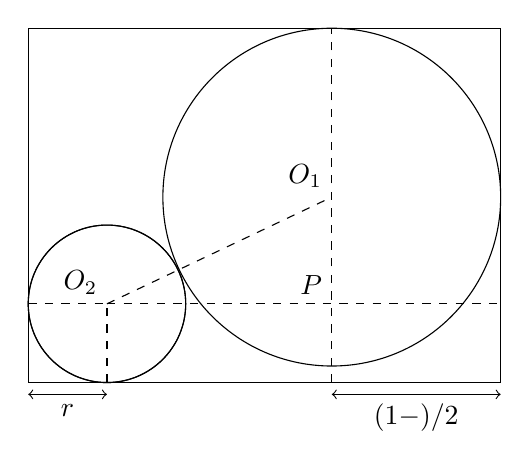
\begin{tikzpicture}[scale=0.5]
		\coordinate (a) at (0,0);
		\coordinate (b) at (12,0);
		\coordinate (c) at (0,9);
		\coordinate (d) at (12,9);
		\coordinate (e) at (2,0);
		\coordinate (f) at (12-4.29,0);
		\draw (0,0) rectangle (12,9);
		\draw (2,2) circle (2cm);
		x=4;
		\draw (12-4.29,9-4.29) circle (4.29 cm);
		\draw[dashed] (2,2) -- (12,2);
		\draw [dashed] (12-4.29,0) -- (12-4.29,9);
		\draw [dashed] (2,2) -- (12-4.29,9-4.29);
		\draw [dashed] (2,0) -- (2,2);
		\draw [dashed] (0,2) -- (2,2);
		\draw (2,2) circle (2cm);
		\node[above left] at (2,2) {$O_2$};
		\node[above left] at (12-4.29,9-4.29) {$O_1$};
		\node[above left] at (12-4.29,2) {$P$};
		\draw[<->] ([yshift=-0.3cm]f) -- ([yshift=-0.3cm]b) node[midway, below]{$(1-\eps)/2$};
		\draw[<->] ([yshift=-0.3cm]a) -- ([yshift=-0.3cm]e) node[midway, below]{$r$};
		\label{Figure 4}
		\end{tikzpicture}
		\caption{Worst case scenario for second biggest sphere in two dimensions.}
		\label{hypersphere}
	\end{figure}
	%\newpage
	% \\\includegraphics[width=10cm]{Images/hypersphere.jpeg}
	
	Let a huge circle of the minimum diameter $1-\eps$ be pushed to the rightmost corner of the augmented box centered at $O_1$. We try and fit a circle of radius $r$ in the bottom-left corner of the box centered at $O_2$. We notice that in 2 dimensions, $O_1 O_2 P$ forms a right triangle. $O_2 P= 1+\eps - r - (1-\eps)/2$, $O_1 P = 1 - r - (1-\eps)/2$, and $O_1 O_2 = r + (1-\eps)/2$. Applying Pythagorean theorem in two dimensions, we get $r=\frac{3}{2} (1+\eps) - \sqrt(2+3\eps)$. In $d$-dimensions, this generalises to $r= \frac{1}{2}+\frac{1}{d-1}+\eps( \frac{1}{2} + \frac{2}{d-1}) -\sqrt{\frac{(1+\eps)^2}{(d-1)^2}+\frac{1-\eps^2}{d-1}}$ and we are done.
\end{proof}

%\begin{restatable}{lemma}{uniqhugeaabs}
\begin{lem}
	\label{uniqhuge}
	For any $0 < \eps \leqslant 1/2d^2$ for all $d \geqslant 2$, there can be at most one hypersphere in $P$ with a diameter larger than $1-\eps$.
	\end{lem}
%\end{restatable}
\begin{proof}
	We always get at most one \textit{huge} hypersphere if the radius calculated in the \Cref{nextrad} is always less than $(1-\eps)/2$. We show that such an $\eps>0$ can always exist regardless of $d$.
	\[\frac{1}{2}+\frac{1}{d-1}+\eps( \frac{1}{2} + \frac{2}{d-1}) -\sqrt{\frac{(1+\eps)^2}{(d-1)^2}+\frac{1-\eps^2}{d-1}} \leqslant (1-\eps)/2 \]
	Analytically solving the quadratic equation, it always holds for \[\eps \leqslant \frac{\sqrt{d^3+3d^2-4d+1}-d}{d^2+3d-1} \leqslant \frac{1}{2d^2}\] where the bound is always positive for all $d \geqslant 2$.
\end{proof}

%\begin{restatable}{theorem}{apxtheoremabs}
\begin{theorem}
	\label{3apx}
	There is a polynomial time $3$-approximation algorithm for the $\mathsf{d-CSK}$ problem.
	\end{theorem}
%\end{restatable}
\begin{proof}
	We show that for values of $\eps<1/2d^2$ as given in \Cref{uniqhuge} we can always partition the augmented bin packing $P$ into three separate packings into unit hypercube bins $B_1, B_2,$ and $B_3$. Let the unique huge hypersphere that intersects both $\ell$ and $\ell'$ be called $C_{huge}$ and remove $C_{huge}$ from all other types of hyperspheres in $P$ as defined earlier. If there is no \textit{huge} hypersphere, then ignore this step. Now note that the set of type 1, type 2, type 3, type 2', type 3', and $C_{huge}$ form a partition of the hyperspheres in $P$.  
	\\We first pack $B_1$ using the same structure as in $P$ with hyperspheres of type 3' and type 2'. This is possible as no hypersphere of type 2' can intersect $\ell$ and we can simply remove the $\eps$-slab to the right of $\ell'$ and we get our bin packing $B_1$. We then pack $B_3$ with hyperspheres of type 2, type 3, and type 1. We then pack the unique hypersphere $C_{huge}$ which has a diameter of at most 1 in a unit bin $B_2$. Note here that we needed to have at most one $C_{huge}$ as the bin width could have been more than 1 even though the huge hyperspheres themselves had a diameter less than 1. We then return the bin out of $B_1, B_2, B_3$ with the most profit.
	\\The running time of this algorithm is clearly polynomial as we get the augmented packing from \Cref{extended-wowa} in polynomial time and the partitioning takes linear time. 
	Since we return the bin with the maximum weight, we return a instance of $\mathsf{d-CSK}$ with a profit of at least $\frac{1}{3} w(\OPT)$. 
\end{proof}

\subsubsection{$(2+\eps)$-approximation algorithm for \(d\leq 8\)} \label{sec:appendix-2-apx}
The main goal of this section is to show that the packings we return for bins $B_1$ and $B_3$ in the $3$-approximation algorithms can in fact be packed into a single bin for $d\leqslant 8$. When there are no \textit{huge} hyperspheres with a diameter greater than $(1-\eps)$, a simple argument for packing in two bins can be made. Also, from \Cref{uniqhuge} we know that for small enough values of $\eps$, there can be at most one \textit{huge} hypersphere.

\begin{restatable}{lemma}{nohugelemmaapx}
	\label{nohuge}
	If there are no \textit{huge} hyperspheres with a diameter bigger than $1-\eps$, then the augmented bin packing $P$ can be partitioned into two unit bin packings $B_1$ and $B_2$.
\end{restatable}
\begin{proof}
	We partition using the same algorithm as in \Cref{3apx} into three unit bins. However the bin that contained the \textit{huge} hypersphere before is now completely empty, so we simply return the other two bins.
\end{proof}

If we have a unique \textit{huge} hypersphere $C_{huge}$, we again show that we can pack $P$ into two different unit bin packings $B_1$ and $B_2$. Let us define another $\eps$-slab $D$ which is parallel to $\ell$ and $\ell'$ and is situated exactly halfway between the two and has $\eps$-width. To use our strategy we need an "empty" $\eps$-slab $S$ in the middle of the augmented bin, which restricts the dimension to $d\leqslant 8$.


\begin{restatable}{lemma}{mindistlemma}
	\label{mindist}
	For $\eps < 1/d^2.2^d$ and $d \leqslant 8$, the distance between any arbitrary type 2 hypersphere and any arbitrary hypersphere of type 2' is at least $\eps$.
\end{restatable}
\begin{proof}
	If the diameter of the hypersphere calculated in \Cref{nextrad} is smaller than $1/2 - \eps$, this is true as the distance between $\ell$ and $D$, $\ell'$ and $D$ is $1/2 - \eps$.   
	\[\frac{1}{2}+\frac{1}{d-1}+\eps( \frac{1}{2} + \frac{2}{d-1}) -\sqrt{\frac{(1+\eps)^2}{(d-1)^2}+\frac{1-\eps^2}{d-1}} \leq 1/4 - \frac{\eps}{2}\]
	This inequality holds true for some positive value of $\eps$ only for $d\leq 8$.  
\end{proof}

\begin{restatable}{theorem}{approxtheorem}
	There is a polynomial time $(2+\eps)$-approximation algorithm for $\mathsf{d-CSK}$ for dimension $d<8$ and $0<\eps<1/4d^2.5^{2d+3}$.
\end{restatable}
\begin{proof}
	We choose $\eps$ small enough from \Cref{uniqhuge} such that there can be at most one \textit{huge} hypersphere of diameter bigger than $1-\eps$. Now, if there are no hyperspheres in the augmented packing $P$ obtained from  \Cref{extended-wowa} with a diameter bigger than $1-\eps$, we proceed to partition and pack $P$ into two augmented unit bins $B_1$ and $B_2$ using \Cref{nohuge}. 
	\\In the case where there is a unique \textit{huge} hypersphere, we choose $\eps$ small enough from \Cref{uniqhuge} such that type 2 and type 2' hyperspheres in $P$ leave an empty $\eps$-strip $D$ between them in the middle of the augmented bin. Now we pack the only huge hypersphere $C_{huge}$ and type 1 hyperspheres into $B_2$. We now can simply remove the strip $D$ and join the segments to get a unit bin packing $B_1$ of hyperspheres of types 2,3,2',3'.
	\\At the end we return packing out of $B_1,B_2$ with maximum weight. This algorithm is clearly polynomial as we get the augmented packing from \Cref{extended-wowa} in polynomial time and the partitioning takes linear time. The algorithm returns an instance of $\mathsf{d-CSK}$ of total weight at least of $\frac{(1-\eps)}{2}w(\OPT)$.
\end{proof}
\end{comment}
%%%%%%%%%
%%%%%%%%%%%

